\documentclass{beamer}
\usepackage[italian]{babel}
\usepackage[utf8]{inputenc}
\usepackage{default}
\usepackage{afterpage}
\usepackage{xcolor}
\usepackage{wrapfig}
\usepackage{caption,subcaption}
\usepackage[font={small,it}]{caption}
\usepackage[font={scriptsize,it}]{subcaption}
\usepackage{bbm}
\usepackage{siunitx}
%\usepackage{movie15}
%\usepackage{multimedia} 
%\newsavebox{\tempbox}
\renewcommand{\vec}[1]{\ensuremath{\boldsymbol{\mathit{#1}}}}
\usetheme{Padova}
\setbeamertemplate{caption}[numbered]
\title{Local Path Planning with Moving Obstacle Avoidance based on Adaptive MPC in ATLASCAR2}
\subtitle{\itshape Tesi di Laurea in Ingegneria dell'Automazione}
\author{Relatore: Prof. Angelo Cenedese\qquad\quad Laureando: Alberto Franco Correlatore: Prof. Vitor Santos}
\date{\vspace{0.4cm}15 Aprile 2019}

\AtBeginSection[]{
	
	\begin{frame}{}
		\nonumber
		\pagecolor{rossoPantano}\afterpage{\nopagecolor}
		\usebeamerfont{title}\vfill\centering
		\usebeamercolor[fg]{title}\insertsectionhead\par%
		\vfill
	\end{frame}
}

\begin{document}

	\maketitle

	\begin{frame}{Progetto ATLAS}
	  \begin{columns}[onlytextwidth,T]
	\begin{column}[c]{0.65\textwidth}
		Questo lavoro di tesi è stato sviluppato all'interno del progetto ATLAS:
		\begin{itemize}
			\item Creato dal gruppo di Automazione e Robotica dell'Università di Aveiro
			
			\item L'obiettivo è sviluppare sistemi per la navigazione autonoma delle automobili %L'obiettivo è studiare e sviluppare sensori avanzati e sistemi attivi per promuovere il controllo autonomo di auto e altre piattaforme
			
			\item 2003 - 2010 Modelli piccola scala\\
			2010 - 2019 Automobili 
			\item 3 LIDAR, 1 Telecamera, 1  Sensore inclinometrico, 1 Unità GNSS
		\end{itemize}
	\end{column}
	\begin{column}[c]{0.33\textwidth}
		\begin{figure}
			\vspace{-3em}
			\centering
			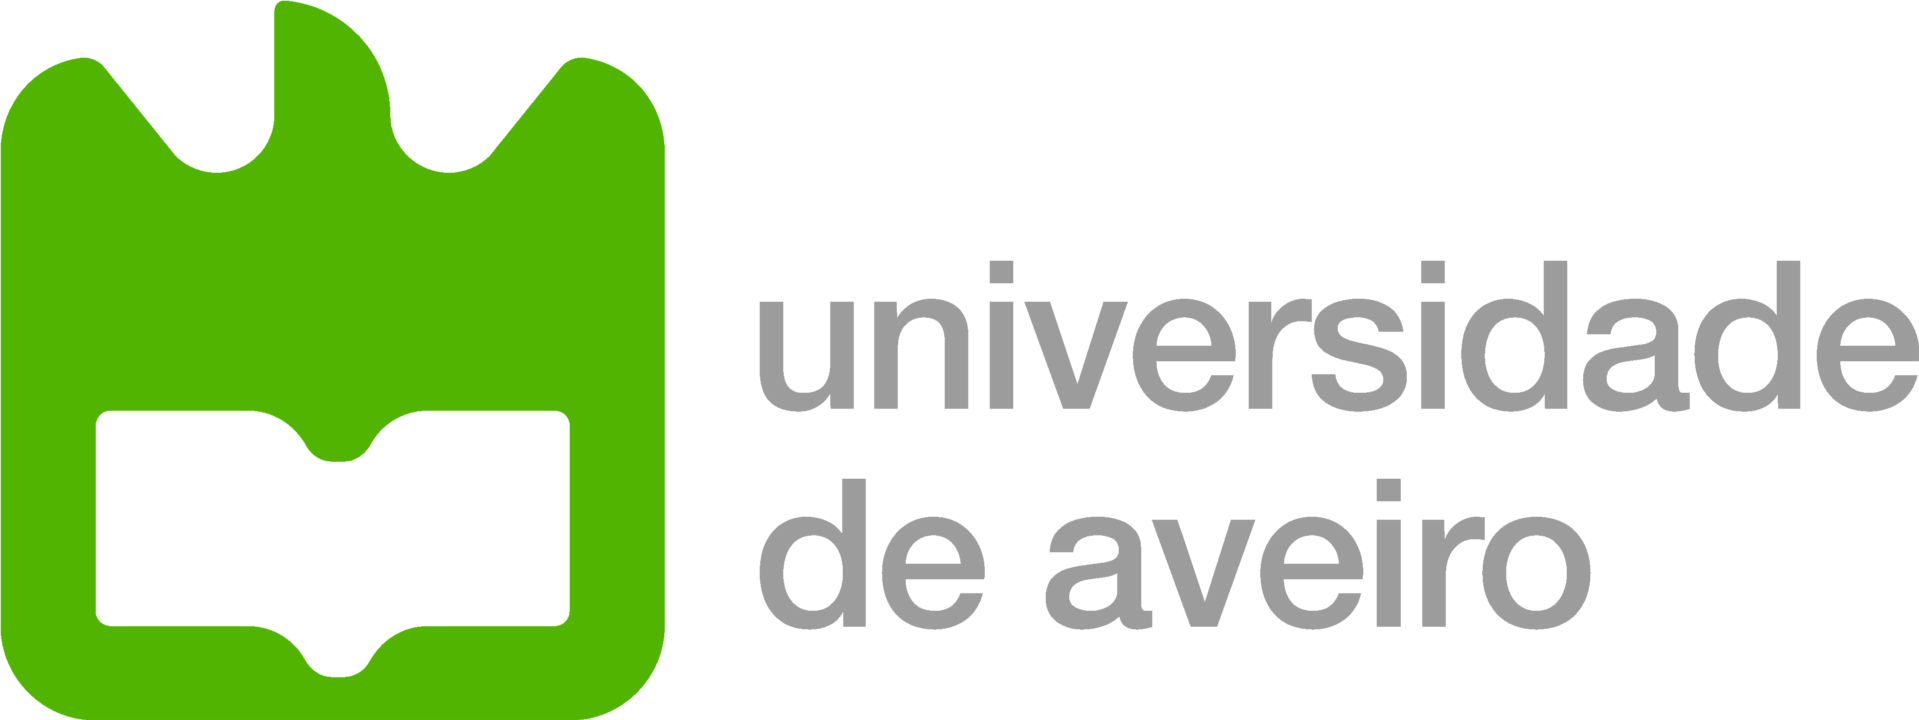
\includegraphics[scale=0.25]{./images/logo_ua.png}
		\end{figure}
		\begin{figure}
			\vspace{-2em}
			\captionsetup{justification=raggedleft}
			\centering
			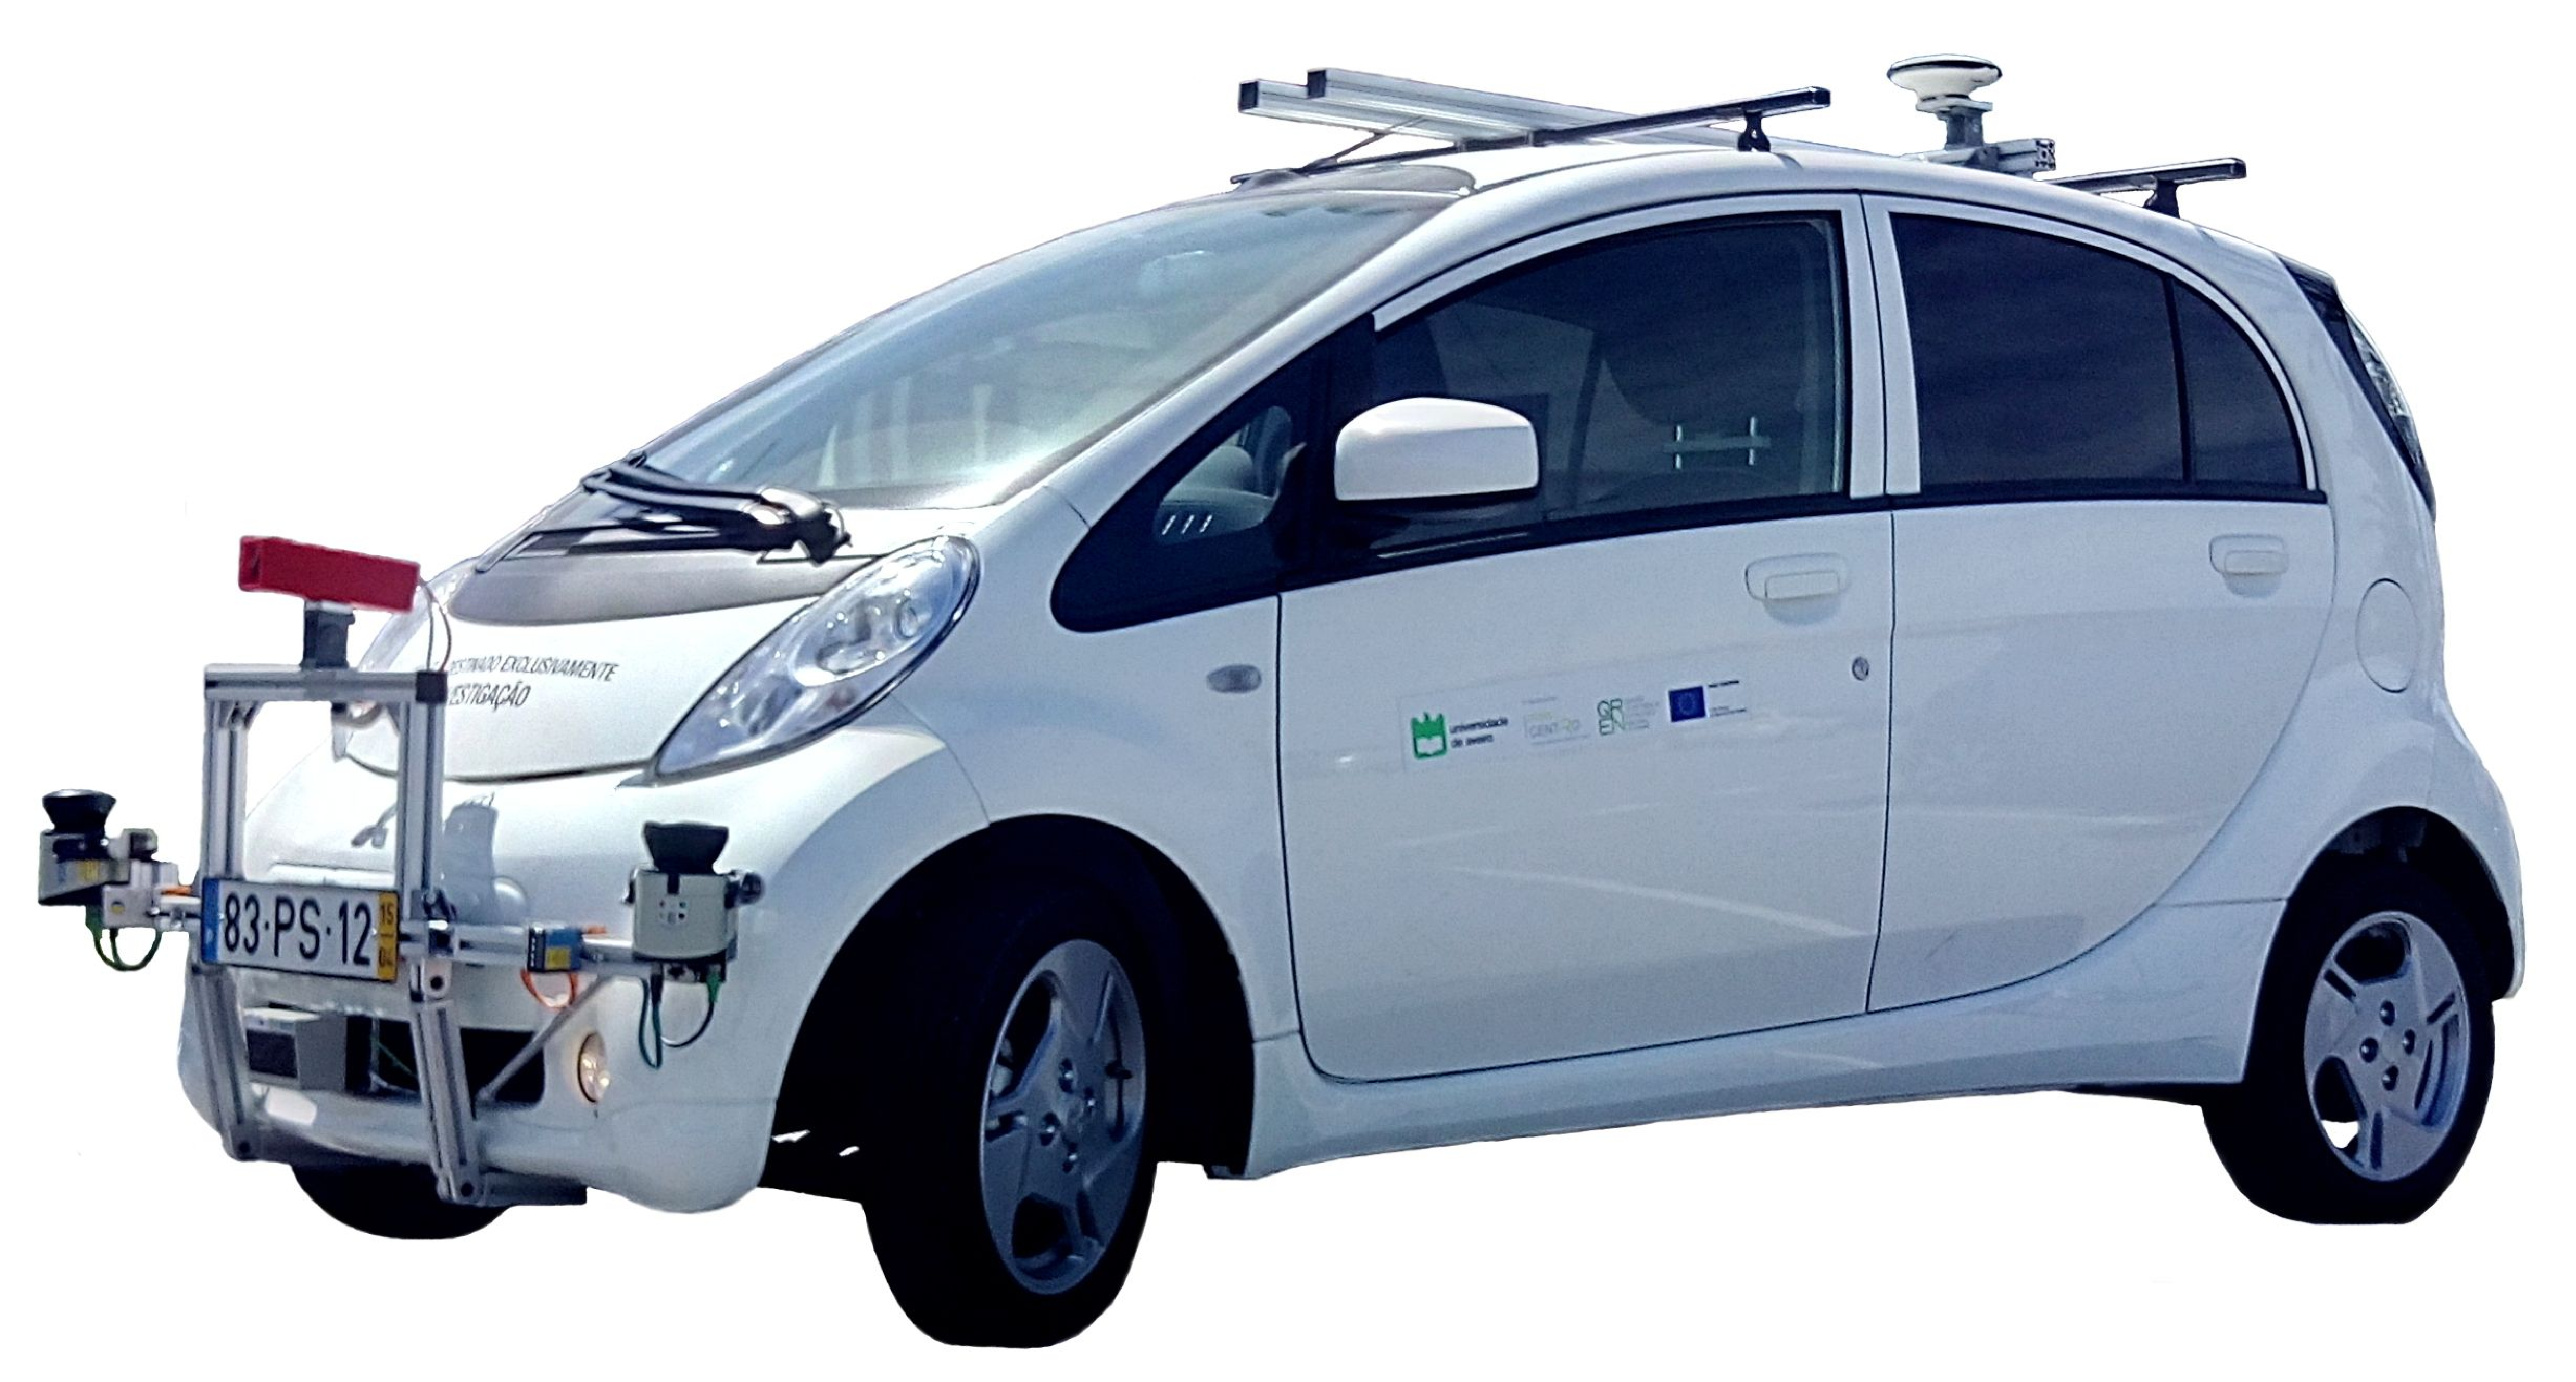
\includegraphics[scale=0.048]{./images/atlascar2.pdf}
			\caption{ATLASCAR2 Mitsubishi iMiEV elettrica del 2015}
		\end{figure}
	\end{column}			
\end{columns}
	\end{frame}

	\begin{frame}{Motivazione e Obiettivi della Tesi}
	Motivazioni:
		\begin{itemize}
			\item Sono stati sviluppati sistemi di navigazione globali
			\item Sistema di pianificazione locale in ambiente statico
		\end{itemize}
	Obiettivi:
		\begin{itemize}
			\item Sistema di anticollisione con ostacoli in movimento
			\item Sistema di assistenza al mantenimento della corsia
		\end{itemize}
	$\Longrightarrow$ Algoritmi basati su ottimizzazione matematica.
	\end{frame}


	\begin{frame}{Model Predictive Control}
		Model Predictive Control:
		\begin{itemize}
			\item tecnica avanzata basata su ottimizzazione matematica
			\item prevede il comportamento futuro utilizzando un modello dinamico LTI
			\item predizioni non esatte - insensibile agli errori di predizione - performance inaccettabili
		\end{itemize}
		$\Longrightarrow$ Tecnica adottata: {\bfseries Adaptive Model Predictive Control}
		\begin{itemize}
			\item adatta il modello di predizione per cambiare le condizioni operative
			\item struttura di modello fissa, ma consente ai parametri del modello di evolvere nel tempo
		\end{itemize}
	\end{frame}
	
	\section{Moving Obstacle Avoidance System {\itshape \large (sistema di anticollisione con ostacoli in movimento)}} % ovvero un sistema di anticollisione con ostacoli in movimento.
		
	\begin{frame}{Formulazione del Problema} 
		Il modello utilizzato è il seguente:
			\begin{equation*}
			\label{eqn:dynamics_model_obstacle_avoidance}
			\left \{ \begin{array}{llll}
			\dot{x} = v\cos(\theta)\\
			\dot{y} = v\sin(\theta)\\
			\dot{\theta} =\dfrac{v}{C_L}\tan(\delta)\\
			\dot{v} =0.5 \cdot T
			\end{array} 
			\right .
			\Longrightarrow 
			\begin{array}{llll}
			\dot{\vec{x}} = \vec{f}(\vec{x},\vec{u})\\
			\vec{y} = \vec{g}(\vec{x},\vec{u})
			\end{array}
			\quad \text{where} \quad 
			\begin{array}{ll}
			\vec{x}=\begin{bmatrix}
			x&y&\theta&v 
			\end{bmatrix}^\intercal
			\\\\
			\vec{u}=\begin{bmatrix}
			T&\delta 
			\end{bmatrix}^\intercal
			\end{array}
			\end{equation*}
			\vspace{-1.5em}
		\begin{columns}[onlytextwidth,T]
			\begin{column}[c]{0.35\textwidth}
				\begin{figure}
					\centering
					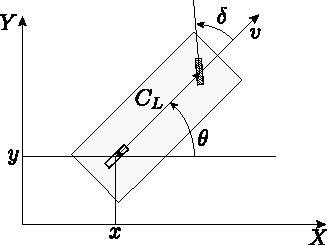
\includegraphics[width=
					\textwidth]{./images/car_model.pdf}
					\caption{Bicycle model}
					\label{fig:car_model}
				\end{figure}
			\end{column}			
			\begin{column}[c]{0.6\textwidth} 
				Per usare l'MPC, il sistema è stato:
				\begin{itemize}
					\item linearizzato con un'approssimazione del primo ordine
					\item discretizzato con il metodo di Eulero (tempo campionamento $T_s$)
				\end{itemize}
				$\Rightarrow$ Ipotesi: tutti gli stati sono misurabili
			\end{column}
		\end{columns}
	\end{frame}
	
	\begin{frame}{Design Adaptive MPC - parte 1} % progettazione dell'algoritmo di anticollisione basato su un controllore MPC adattivo.
	\vspace{-1.3em}
	\begin{columns}[onlytextwidth,T]
		\hspace{-2.4em}
		\begin{column}[c]{0.72\textwidth}
		\begin{figure}[!h]
			\centering
			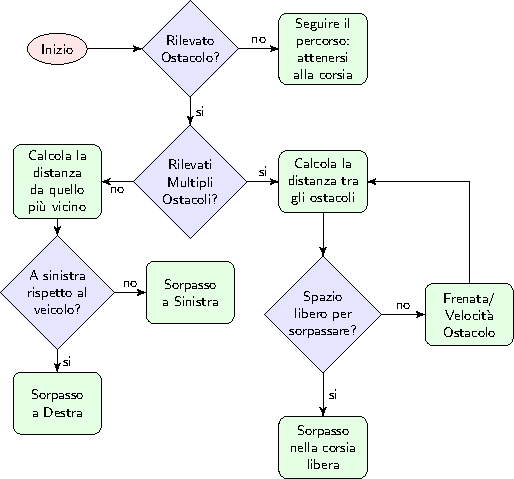
\includegraphics[width=
			\textwidth]{./images/flowchart/flowchart.pdf}
			\captionsetup{singlelinecheck = false, format= hang, justification=raggedright,}
			\caption{Algoritmo decisionale}
			\label{fig:flowchart}
		\end{figure}
		\end{column}	
		\hspace{1em}		
		\begin{column}[c]{0.4\textwidth}
		L'ATLASCAR2 deve:
		\begin{itemize}
		\item seguire una velocità di riferimento
		\item rimanere nel mezzo della corsia centrale
		\end{itemize}
		\vspace{1.4em}
		Per definire l'area del sorpasso usiamo i seguenti vincoli di ingresso/uscita:
		\begin{equation*}
		\label{eqn:mixed_IO_constraints}
		\vec{E}\vec{u}+\vec{F}\vec{y}\leq \vec{G}
		\end{equation*}
		dove $\vec{E},\vec{F}$ e $\vec{G}$ sono aggiornate ogni $T_s$
		\end{column}
	\end{columns}
	\end{frame}
	
	\begin{frame}{Design Adaptive MPC - parte 2} % progettazione dell'algoritmo di anticollisione basato su un controllore MPC adattivo.
		\hspace{-2em}
		{\vspace{5em} L'area del sorpasso è definita come $\vec{E}\vec{u}+\vec{F}\vec{y}\leq \vec{G}$ dove: $\quad\Rightarrow\vec{E}=\vec{0}_{5\times2}$}
		\begin{columns}[onlytextwidth,T]
			\hspace{-1.5em}
			\begin{column}[c]{0.73\textwidth}
				\vspace{-5.6em}
				\begin{figure}[!t]
					\centering
					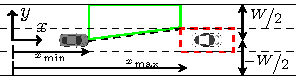
\includegraphics[width=0.9\columnwidth]{./images/constraint/constraint.pdf}
					\caption{Vincoli nel sorpasso a sinistra.}
					\label{fig:constraint}
				\end{figure}
				\vspace{-0.8em}
				\hspace{-0.5em} Sono stati definiti i seguenti vincoli:
				\begin{enumerate}
				\item limite superiore coordinata $y$
				\item limite inferiore coordinata $y$
				\item linea veicolo-angolo della zona di sicurezza
				\item limite destro coordinata $x$
				\item limite sinistro coordinata $x$
				\end{enumerate}
			\end{column}
			\begin{column}[c]{0.34\textwidth}
				\vspace{-6em}
				\begin{equation*}
				\begin{array}{lll}
				\hspace{-0.5em}\Rightarrow\vec{F}=\begin{bmatrix}
				0&1&0&0\\
				0&-1&0&0\\
				cS&-1&0&0\\
				1&0&0&0\\
				-1&0&0&0\\
				\end{bmatrix}\\\\
				\quad\Rightarrow\vec{G}=
				\begin{bmatrix}
				W/2\\W/2\\-cI\\x_{\max}\\x_{\min}
				\end{bmatrix}
				\end{array}
				\end{equation*}
			\end{column}
		\end{columns}
	\end{frame}
	
	\begin{frame}{Risultati Simulativi}
		\begin{figure}								
		\href{run:./video/animation_one_obstacle_left_overtaking.avi}{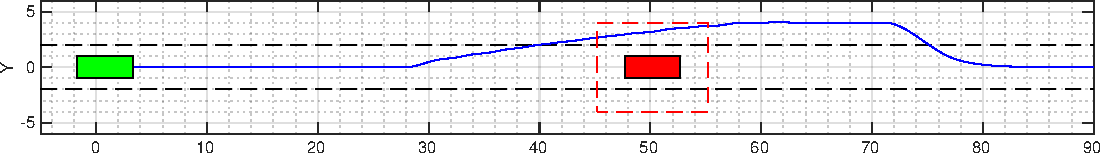
\includegraphics[width=\textwidth]{./images/one_obstacle_right_overtaking/overtaking_pres.pdf}}
		\caption{\href{run:./video/animation_one_obstacle_left_overtaking.avi}{Sorpasso a sinistra di un ostacolo in movimento (animazione)}}
		\label{fig:un_ostacolo}
		\vspace{-1.5em}
		\end{figure}
		\begin{figure}
		\href{run:./video/animation_6_obstacles.avi}{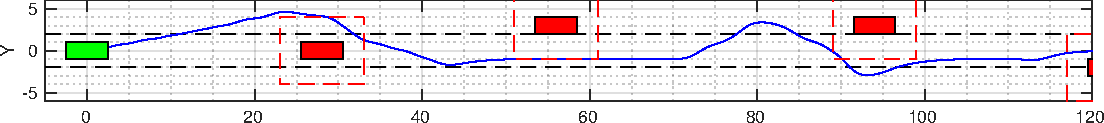
\includegraphics[width=\textwidth]{./images/6_obstacles/6_obstacles_pres.pdf}}
		\caption{\href{run:./video/animation_6_obstacles.avi}{Sorpasso di 6 ostacoli in movimento (animazione)}}
		\label{fig:sei_ostacoli}
		\vspace{-1.5em}
		\end{figure}
		\begin{figure}
		\href{run:./video/animation_braking_overtaking.avi}{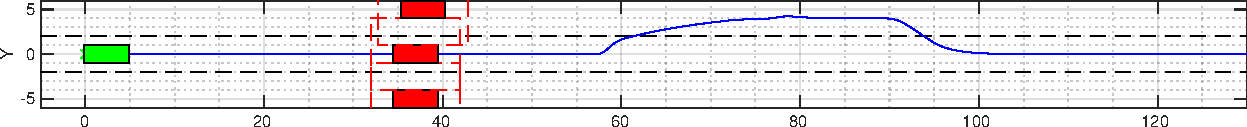
\includegraphics[width=\textwidth]{./images/three_obstacles_no_overtaking/braking_pres.pdf}}
		\caption{\href{./video/animation_braking_overtaking.avi}{Frenata e sorpasso di 3 ostacoli in movimento (animazione)}}
		\label{fig:frenata}
		\end{figure}
	\end{frame}
	
	\section{Lane Following System \qquad\qquad{\itshape\large(sistema di assistenza al mantenimento della corsia)}}  % ovvero un sistema di assistenza al mantenimento della corsia.
	
	\begin{frame}{Formulazione del Problema}
		\vspace{-2.5em}
		\begin{columns}[onlytextwidth,T]
			\hspace{-2.5em}
			\begin{column}[c]{0.5\textwidth}
			\begin{figure}[!h]
			\centering
			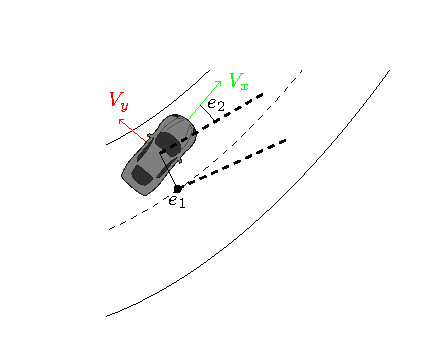
\includegraphics[width=\columnwidth]{./images/laneFollowing/laneFollowingPres.pdf}
		\end{figure}
		\centering
		\textbf{Dinamica dei Sensori\\}
		$e_1$ = Deviazione Laterale\\
		$e_2$ = Tasso di imbardata relativo\\
		$\big\Downarrow$\\
		Devono essere guidati a zero
			\end{column}
			\begin{column}[c]{0.65\textwidth}
				\textbf{Obiettivo}: il veicolo deve seguire la linea centrale, con una velocità di riferimento.\\
				\vspace{2em}
				\textbf{Dinamica del veicolo}:
				\begin{itemize}
					\item Longitudinale $\rightarrow$ Funzione di trasferimento del primo ordine.
					\item Laterale $\rightarrow$ Bicycle model parametrizzato
				\end{itemize}
				\vspace{2em}
				\centering
				\textbf{Modello complessivo}: viene discretizzato secondo Eulero, tiene conto dell' intera dinamica e degli errori.
			\end{column}
		\end{columns}
		
		
	\end{frame}
	
	\begin{frame}{Design Adaptive MPC} % progettazione dell'algoritmo di mantenimento della corsia basato su un controllore MPC adattivo.
		\begin{figure}[!h]
			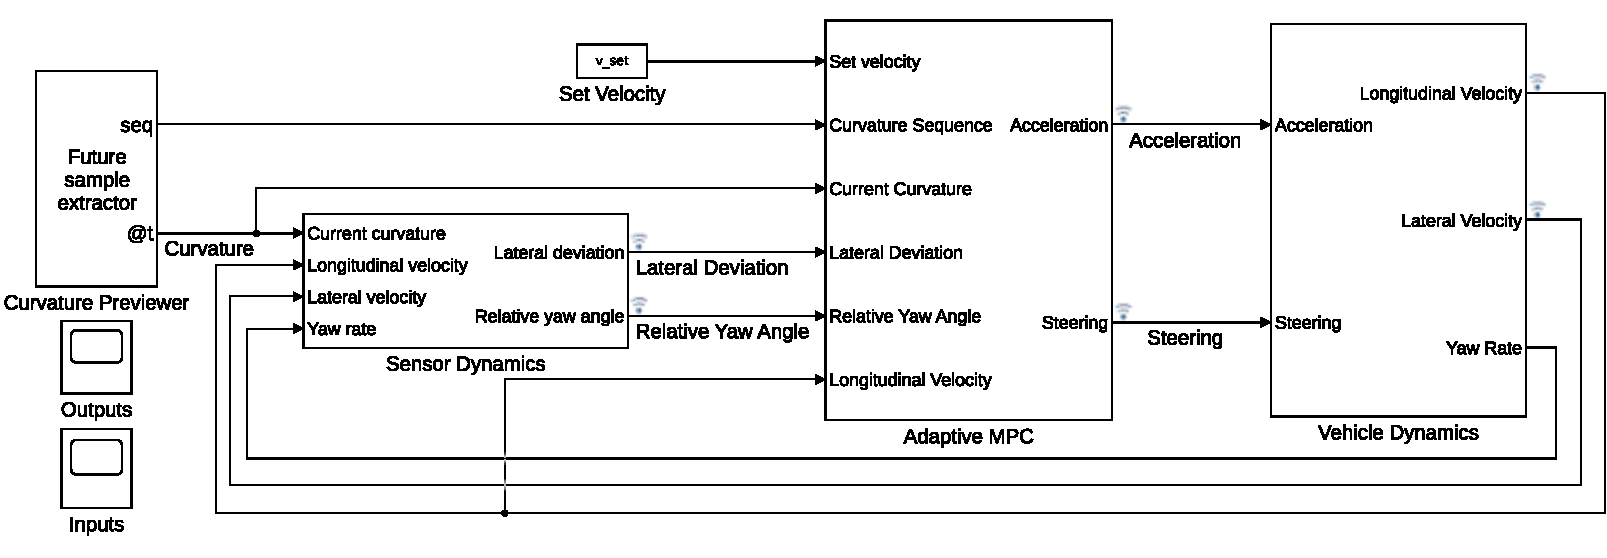
\includegraphics[width=\textwidth]{./images/lane_following_AMPC.pdf}
			\caption{Schema di controllo per il mantenimento della corsia}
			\label{fig:scheme_lane_following}
		\end{figure}
		\textbf{Adaptive MPC:} modello predittivo con 6 stati, 3 output, 2 variabili indipendenti. Abbiamo vincolato l'accelerazione e l'angolo di sterzata per una guida più confortevole.
	\end{frame}

	\begin{frame}{Risultati Simulativi - parte 1}
		\vspace{-1.4em}
		\begin{columns}[onlytextwidth,T]	
			\begin{column}[c]{0.5\columnwidth}
				\begin{figure}[!h]
					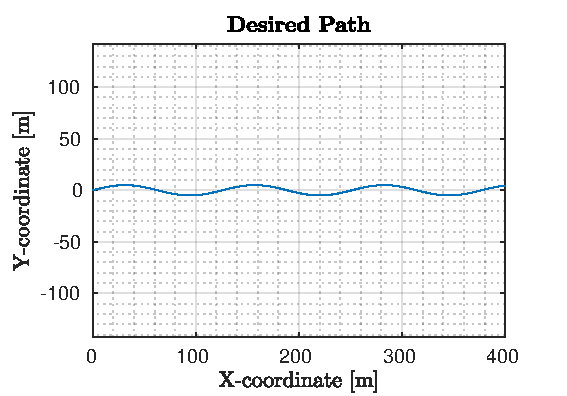
\includegraphics[width=0.92\columnwidth]{../../MATLAB/lane_following/figure/Reference.pdf}
					\vspace{-0.5em}
					\caption{Traiettoria Sinusoidale}	
				\end{figure}
				\begin{figure}[!h]
					\vspace{-2.4em}
					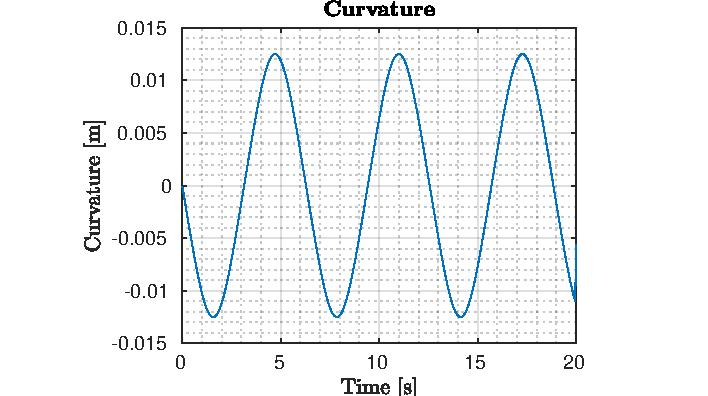
\includegraphics[width=0.92\columnwidth]{../../MATLAB/lane_following/figure/Curvature.pdf}
					\vspace{-0.5em}
					\caption{Curvatura}
				\end{figure}
			\end{column}
			\begin{column}[c]{0.55\columnwidth}
				Esempio: \textbf{Percorso Sinusoidale}
				\begin{equation*}
				\begin{array}{ll}
				X_\text{ref}=V_x\cdot t,\quad t\in[0,20]\SI{}{s}\\ Y_\text{ref}=5\sin(X_\text{ref}/20) 
				\end{array}
				\end{equation*}
				Ipotesi:\\
				{\hspace{1em}
				$\rightarrow$ Velocità iniziale \SI{15}{m/s}\\
				\hspace{1em} $\rightarrow$ Velocità di crociera \SI{20}{m/s}\\}
				\vspace{1.5em}
				Calcoliamo la \textbf{Curvatura}:
				\begin{equation*}
				\label{eqn:curvature}
				\kappa=\frac{x'y''-x''y'}{(x'^2+y'^2)^\frac{3}{2}}
				\end{equation*}
				che sarà il riferimento da inseguire
			\end{column}	
		\end{columns}		
	\end{frame}
		
	\begin{frame}{Risultati Simulativi - parte 2}	
		\vspace{-2.4em}
		\begin{columns}[onlytextwidth,T]
			\begin{column}[c]{0.5\columnwidth}
				\begin{figure}[!h]
				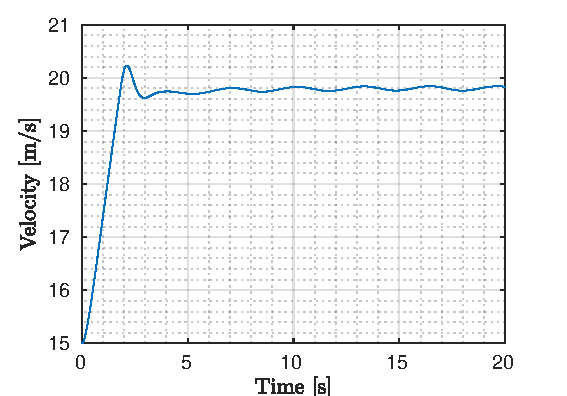
\includegraphics[width=0.92\columnwidth]{../../MATLAB/lane_following/figure/LongitudinalVelocityVsTime.pdf}
				%\captionsetup{font=scriptsize}
				\vspace{-0.5em}
				\subcaption*{Velocità Longitudinale $V_x$}
				\end{figure}
				\begin{figure}[!h]
				\vspace{-3em}
				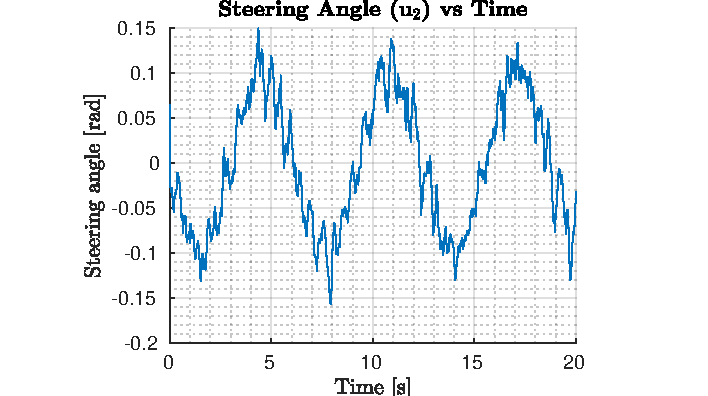
\includegraphics[width=0.92\columnwidth]{../../MATLAB/lane_following/figure/SteeringAngleVsTime.pdf}
				%\captionsetup{font=scriptsize}
				\vspace{-0.5em}
				\subcaption*{Angolo di Sterzata $u_2$}
				\end{figure}	
			\end{column}		
			\begin{column}[c]{0.5\columnwidth}
				\begin{figure}[!h]
				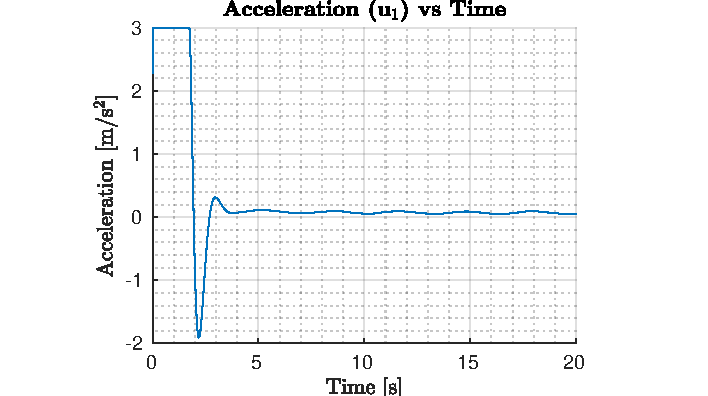
\includegraphics[width=0.92\columnwidth]{../../MATLAB/lane_following/figure/AccelerationVsTime.pdf}
				%\captionsetup{font=scriptsize}
				\vspace{-0.5em}
				\subcaption*{Accelerazione $u_1$}	
				\end{figure}
				\begin{figure}[!h]
				\vspace{-3em}	
				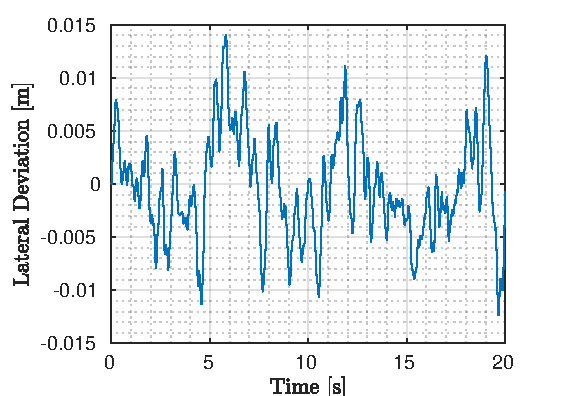
\includegraphics[width=0.92\columnwidth]{../../MATLAB/lane_following/figure/LateralDeviationVsTime.pdf}
				%\captionsetup{font=scriptsize}
				\vspace{-0.5em}
				\subcaption*{Deviazione Laterale $e_1$}
				\end{figure}
			\end{column}
		\end{columns}		
	\end{frame}
	
	\begin{frame}{Conclusioni e Sviluppi Futuri}
		\begin{columns}[onlytextwidth,T]
			\begin{column}[c]{0.75\textwidth}
				\textbf{Conclusioni}:			\begin{itemize}
					\item Sistema di anticollisione in ambiente dinamico (ostacoli in movimento)
					\item Sistema di assistenza al mantenimento della corsia (Lane Keeping Assist)
				\end{itemize}
				\textbf{Sviluppi futuri}:
				\begin{itemize}
					\item Combinazione dei due metodi in un unico schema di controllo
					\item Implementazione in ambiente ROS-Gazebo
					\item Uso di dati reali collezionati dai sensori dell'ATLASCAR2 per testare gli algoritmi sviluppati
				\end{itemize}
			\end{column}
			\begin{column}[c]{0.20\textwidth}
				\begin{figure}
					\vspace{-3em}
					
\includegraphics[width=
					\textwidth]{./images/GAZEBO.png}
				\end{figure}
				\begin{figure}
					\vspace{-3em}
					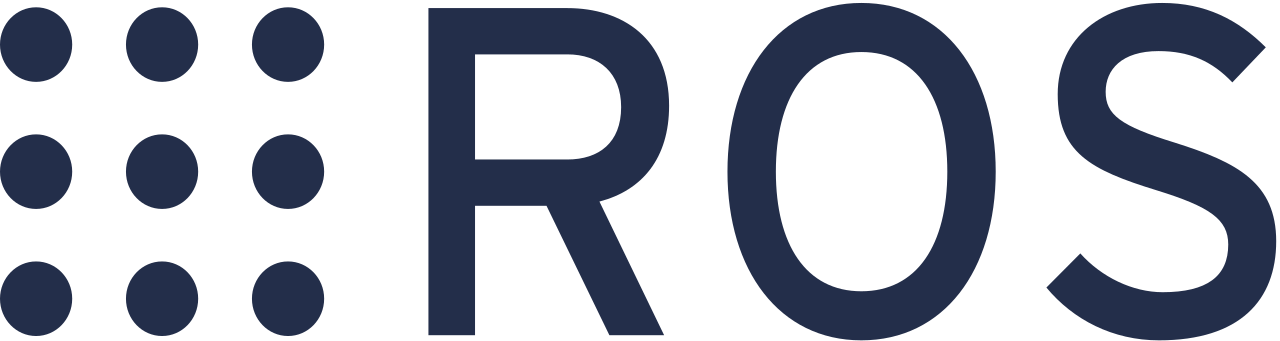
\includegraphics[width=
					\textwidth]{./images/ROS.png}
				\end{figure}
			\end{column}			
		\end{columns}
	\end{frame}

\end{document}
